%%% Local Variables: 
%%% mode: latex
%%% TeX-master: "../KanjiHWR"
%%% End: 

\chapter{On-Line Handwriting Recognition}
\label{chap:onlinehwr}

%\minitoc

%\begin{itemize}
%\item Warum: Um Ueberblick ueber HWR-Techniken zu verschaffen
%\item Nutzen: Leser kann sich in HWR-Materie eindenken.
%\item Was: Allg. Info ueber HWR. "Wie geht das ueberhaupt?"
%\item Wie: Wiss. Report. / Zusammenfassung. Vergleich.
%\end{itemize}

\section{Introduction}
\label{sec:onlinehwrintroduction}

%xxx: see plamondon2000 intro
%xxx: see plamondon2000 2: different disciplines
%xxx: see santosh2009: introduction for related stuff

Handwriting is a very personal skill to individuals. It consists of graphical
marks on a surface and can be used to identify a person. Communication is the main purpose and this is achieved by drawing letters or other 
\emph{graphemes}, which in turn represent parts of a language.
The characters have a certain basic shape, which must be recognisable
for a human in order for the communication process to function.
There are rules for the combination of letters, which have the ability - if
known to the reader - to help recognise a character or word.

Handwriting was developed as a means of communication and to expand one's own
memory. With the advent of each new technologies the question arose, 
if handwriting was going to survive. However, the opposite seems to be the 
truth: For example, the printing press increased the number of documents
available and therefore increased the number of people who learnt to read
and write. Through the increased rate of alphabetisation, naturally there was
an increased use of handwriting as a means of communication.

In various situations handwriting seems much more practical than typing on a
keyboard. For instance children at school are using notepads and pencils or
ink pens, which are regarded as a better tool to teach writing by German 
teachers. Therefore it can be concluded that there is little danger of
the extinction of handwriting as a communication tool. In fact, as 
the length of handwritten messages decreases, the number of people using 
handwriting increases \shortcite{Plamondon2000}.

\section{Handwriting Features}
\label{sec:handwritingfeatures}

Any script of any language has a number of features. The fundamental 
characteristic of a script is that the differences between the features
of different characters are more decisive than the different features of 
drawing variants of the same letter in individual handwriting styles.
There might be exceptions, because \emph{0} (number between '-1' and '1') and 
\emph{O} (letter between 'n' and 'p') or \emph{1} (number between '0' and '2') 
and \emph{I} (letter between 'h' and 'j') respectively, can be written alike. 
However, in those cases, context makes clear which one was intended by the 
writer. Despite the exception, written communication can only work with that
fundamental quality \shortcite{Tappert1990}.

\subsection{Handwriting Properties of Latin Script}
\label{sec:handwritingpropertieslatin}

In the Latin script we have 26 letters, each of which has two variants, 
a capital and a lowercase variant. When writing a character 
in the Latin script, there are four main areas, in which the character 
can reside. All characters have their main part between a top line and a 
ground line. There is also a middle line. Capital characters stretch out to use
the full space between the ground line and the top line, whereas lowercase 
characters usually use the space between the ground line and the middle line. 
Some lowercase characters (like lowercase \emph{b, d, f, h, k, l, t}) have an
ascender and use the area above the middle line as well, 
some lowercase characters have a descender and use the area below the ground 
line (like lowercase \emph{g, j, p, q, y}). In handwritten cursive script, 
there are writing variants where also some lowercase letters (\emph{f, z}) and
certain uppercase characters (\emph{G, J}) expand below the ground line.
For all latin-based alphabets, usually one character is finished before the 
next one starts, however, there are exceptions:
In cursive handwriting, the dots on \emph{i} and \emph{j} and the crosses
of \emph{t} might be delayed until the underlying portions of all 
the characters of the word are completed. 
Figure~\ref{fig:expandingcursiveletters} shows examples of letters that expand 
below the ground line with their descender or stretch up to the top line with
an ascender.

XXX Graphic with example of expanding cursive letters here.

\begin{figure}[htbp]
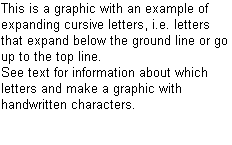
\includegraphics[scale=0.5]{images/expandingcursiveletters.png}
\caption{Expanding cursive letters}
\label{fig:expandingcursiveletters}
\end{figure}

\subsection{Handwriting Properties of East Asian Scripts}
\label{sec:handwritingpropertieseastasian}

% xxx: see tappert1990 IV handwriting properties and recognition problems
Generally, a handwriting is a formed of a number of strokes, that are drawn
in a time sequence. Opposed to the latin-based alphabets, consider Chinese and
Japanese script. Chinese has a larger alphabet, up to 50.000 characters, 
3.000-5.000 of which are in active use. There are also two writing styles,
block style - which corresponds to printed characters in Latin alphabets,
even if handwritten. The other style is cursive style. In block style the
individual parts of the character are usually written in proper stroke order,
and abide by the proper stroke number. In cursive style the characters are
written faster, with less care and don't necessarily abide to stroke
number or order. In fact, they are usually written with fewer strokes,
connecting some block-style strokes by using simpler radical 
shapes \shortcite{Tappert1990}.

In Japanese, three different scripts are in active use at the same time,
mixed and next to each other. They are called \emph{Hiragana} (\cjk{ひらがな}), 
\emph{Katakana} (\cjk{カタカナ}) and \emph{Kanji} (\cjk{漢字}).
Hiragana and Katakana are syllabic alphabets, each containing 46 characters
(see section~\ref{sec:kana}), whereas Kanji are essentially the Chinese 
\emph{Hànzì} (\cjk{汉字}) characters as they were imported into the Japanese 
language (see section~\ref{sec:ahorthistoryofjapanesewritingsystem}).

The different scripts can even be blended with each other within one word. 
Take for instance the verb '\cjk{食べる}' (pron. \emph{/taberu/}, 
Eng. \emph{to eat}). 
The first character '\cjk{食}' is a Kanji character, pronounced \emph{/ta/}, 
which also bears the meaning of the word. The second and third characters 
are the Hiragana characters '\cjk{べ}' \emph{be} and '\cjk{る}' \emph{ru}, 
which are there for conjugation only as well as for phonetic reasons. 
Without them, the character '\cjk{食}' still bears the meaning of the concept 
\emph{eat}, but the character alone does not result in the verb \emph{taberu}.

\section{Automated Recognition of Handwriting}
\label{sec:autorecoofhandwriting}

\subsection{Short History of Handwriting Recognition}
\label{sec:shorthistoryofhwr}

\emph{Handwriting recognition} (HWR) as a technological discipline performed 
by machines has been around for many years. The quality of the systems 
recognising handwriting has improved over the decades. It is the key 
technology to pen-based computer systems. The first research papers 
concerned with \emph{pattern recognition} on computers were published 
in the late 1950'ies, \emph{Handwriting recognition} as an individual subject in 
the early 1960'ies. \shortcite{Goldberg1915} describes in a US Patent
a machine that can recognise alphanumeric characters as early as 1915. 
However, despite the surprise of how early such a device was invented,
it should be taken into consideration that that was before the times 
of modern computers, therefore the methods he employs are quite different 
from the algorithms used after the advent of computers, more concretely, 
computers with screens. 

\shortcite{Tappert1990} describe in their review the development of 
handwriting recognition, which was a popular research topic in the early 
1970'ies and then again in the 1980'ies, due to the increased availability 
of pen-input devices.  Generally speaking, handwriting recognition (HWR) 
involves automatic conversion of handwritten text into a machine readable 
character encoding like ASCII or UTF-8. Typical HWR-environments include 
a pen or stylus that is used for the handwriting, a touch-sensitive surface, 
which the user writes on and a an application that interprets the strokes 
of the stylus on the surface and converts them into digital text. 
Usually, the writing surface captures the x-y coordinates of the stylus 
movement.

\subsection{Pattern Recognition Problems}
\label{sec:patternrecognitionproblems}

%xxx: was ist das generelle problem?
%xxx: welche probleme treten dabei auf?
%xxx: related problems: see liujaegernakagawa2004 1.1
%xxx: write something about the problems of different scripts here, 
%xxx: too, as in tappert1990 IV: problems.

The general problem of \emph{pattern recognition} is to take a non-symbolic 
representation of some pattern, like mouse or pen coordinates and transform
it into a symbolic representation like a \emph{rectangle} with its coordinates,
or in the case of handwriting recognition, a character. Pattern recognition is 
a symbol manipulation procedure, that tries to generate discrete structures or sub-sets of discrete structures. Some see it as a game theory problem, 
where machine 'players' try to match the interpretation of an input produced 
by machine 'experts' \shortcite{Zanibbi2005}.

\subsubsection{Related Problems}
\label{sec:relatedproblems}

There are several related problems, the recognition of equations, line 
drawings and gestures symbols. The recognition of language symbols includes 
the different large alphabets of Chinese, the different scripts of Japanese, 
alphabetic scripts like Greek, or Arabic and other non-alphabetic scripts like
the Korean  Hangul, but also various writing styles of the latin-based 
alphabets, and diacritics that are used to denote pronunciation variants in 
different languages using Latin script, like Turkish or Vietnamese.

Other Problems that are related to handwriting recognition include for example
mathematical formula recognition, where mathematical formulae are analysed and 
put into a computable format \shortcite{ChanYeung2001}. In diagram recognition 
both the characters and the diagram layout are recognised 
\shortcite{Blostein1999}.

\subsubsection{Problem of Similar Characters}
\label{sec:similarcharacters}

\begin{figure}[htbp]
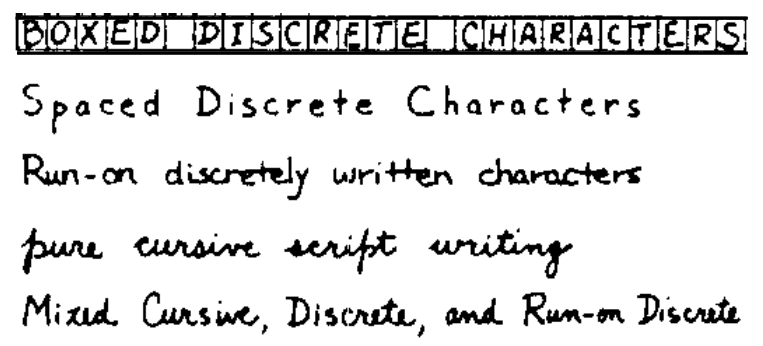
\includegraphics[scale=0.5]{images/differentHandwritingStyles.png}
\caption{Different handwriting styles}
\label{fig:differenthandwritingstyles}
\end{figure}

XXX remake fig 2. in Tappert1990 which he had stolen from his reference 240

There are several subproblems to the task of pattern recognition of a character.
Different styles of handwriting after~\shortcite{Tappert1990} can be seen in 
figure~\ref{fig:differenthandwritingstyles}.
The scripts toward the bottom of figure~\ref{fig:differenthandwritingstyles} 
are harder to recognise. In the case of boxed discrete characters, segmentation 
is done for the machine by the user. Run-on discrete characters are easier to 
recognise than pure cursive handwriting, because there is a pen-up and 
pen-down between each character. In cursive handwriting, segmentation 
between the characters becomes a more difficult task. Some parts of the writing
may be delayed, like the crosses of \emph{t} or the dots on \emph{i} or \emph{j}.
Besides the segmentation, the discrimination of shapes is often not trivial.
Humans may or may not be able to decipher somebody else's handwriting and clearly
distinguish between, say \emph{U-V}, but most of the times, context helps with 
that task. Other characters have similar shapes, too, like \emph{C-L}, \emph{a-d}
and \emph{n-h}. Confusion can arise between characters and numbers like 
\emph{O-0}, \emph{I-1}, \emph{l-1}, \emph{Z-2}, \emph{S-5}, \emph{G-6}, 
\emph{I-1}, \emph{Z-2}. Lowercase and uppercase are hard to distinguish in the
cases of \emph{C-c}, \emph{K-k}, \emph{O-o}, others are mainly distinguished 
by their position relative to the base line of the rest of the text: 
\emph{P-p}, \emph{Y-y}. Therefore, context helps the human reader to identify
the correct character. This could be used as an advantage in automated pattern
recognition, as well. However, the other characters nearby would have to be
recognised first, which creates a (solvable) hen and egg problem.
In the Japanese script the problem is taken to another dimension. 
Consider \cjk{本}~(root) and \cjk{木}~(tree) those two characters are only a 
very basic sample of characters that might lead to confusion of the different 
symbols. However, due to the hierarchical organisation of the characters 
with their radicals
(see section~\ref{sec:japanesewritingsystemtoday}) there are many more shapes 
that look very much alike. From the shape recognition perspective, 
minor changes to the shape of a character can change its meaning drastically.
Compare \cjk{嘸}~(how, indeed), \cjk{撫}~(stroke, pat), \cjk{蕪}~(turnip) and
\cjk{憮}~(disappointment). They all contain the radical 
\cjk{無}~(nothingness, none), which doesn't seem to have any semantic connection
with the characters, however, it can be seen as the main radical in those 
characters.

\subsection{Hardware Requirements}
\label{sec:hardwarerequirements}
%xxx: see santosh2009 basic tools / techniques / digitiser technology, 

In order to perform on-line handwriting recognition, the handwriting needs to 
be captured in some way. Special hardware is necessary to perform the task of
capturing both the x-y coordinates and the time information of the handwriting
input device.

Several different hardware commercial products are available in order to
capture the x-y coordinates of a stylus or pen. Graphics tablet like the
products of the Wacom Co., Ltd.\footnote{www.wacom.com} are popular input
devices for hand motions and hand gestures. The use of pen-like input devices 
has also been recommended, since 42\% of mouse users report feelings of 
weakness, stiffness and general discomfort in the wrist and hand when 
using the mouse for long periods \shortcite{Woods2002}. 
The sampling rates of digital pens are usually around 50-200 Hz. The higher the
sampling rate the finer the resolution of the resulting co-ordinates,
which leads to more accurate measurement of fast strokes. 

Moreover there are PDAs and Tablet PCs, where the writing surface serves 
as an output device, i.e. an display at the same time.
If the pen capturing area is transparent and has an instantaneous display behind
that shows immediately whatever input the user drew with the stylus,
a high level of interactivity can be reached \shortcite{Santosh2009}. 
These displays include touch screens, which are a newer development. 
New generation mobile phones like the notorious iPhone from Apple Inc. 
also contain touch-displays, but for those it is more common to be 
operated without a stylus. For the task of handwriting recognition, 
a stylus can be regarded as the more natural device, 
since people usually write with pens on paper,
therefore a stylus on a display seems more natural than using a 
finger on a display for writing. 
In order to interpret user gestures, an input given directly with the fingers
is a more natural option. Gestures for zooming into digital pictures, 
or turning to the next page of a document are interpreted on these devices.

Another rather new development are real-ink digital pens. With those, 
a user can write on paper with real ink, and the pen stores the 
movements of the pen-tip on the paper. The movements are transferred to a 
computer later. 
It can be expected that with technologies like Bluetooth it may be possible 
to transfer those data in real-time, not delayed.
In a fairly new development accelerometer technology has been used 
for handwriting recognition, using a mobile phone as a device to write 
in the air \shortcite{Agrawal2009}. That approach can be regarded as an area 
that is only loosely related to classical handwriting recognition, 
as the phone stores an image of the strokes in the air that were measured
by the accelerator device, but does not transform the strokes into characters.

%xxx: if you want to add more technical details here, 
%see Santosh2009:Digitizer Technology. :xxx

\subsection{Recognition vs Identification}
\label{sec:recognitionvsidentification}

Handwriting recognition is the task of transforming a spatial language 
representation into a symbolic representation. In the English language
(and many others) the symbolic representation is typically 8-bit ASCII.
However, with \emph{Unicode} being around for more than a decade now,
storage space on hard disks not being as much of an issue any more and
\emph{RAM} being readily available to the Gigabytes, it has become more 
common to use a \emph{UTF-8}  encoding, which is a variable-length character 
encoding for Unicode \shortcite{Unicode2000}.
Akin disciplines to handwriting recognition are 
\emph{handwriting identification}, which is the task of identifying the author
of a handwritten text sample from a set of writers, assuming that each
handwriting style can be seen as individual to the person who wrote it.
The task of \emph{signature verification} is to determine if a given signature
stems from the person who's name is given in the signature.
Thus, handwriting identification and verification can be used for 
analysis in the field of jurisdiction. They determine the individual features
of a handwritten sample of a specific writer and compare those
to samples given by a different or the same writer. By analysing those 
features one can find out if a piece of handwritten text is authentic or not.

\subsection{Interpretation of Handwriting}
\label{sec:interpretationofhandwriting}

Handwriting recognition and interpretation are trying to filter out the 
writer-specific variations and extract the text message only. This conversion
process can be a hard task, even for a human. Humans use context knowledge
in order to determine the likeliness of a certain message in a certain context.
For instance, a handwritten message on a shopping list that could be read
as \emph{bread} or \emph{broad} due to the similarities of the characters 
for 'e' and 'o' in some cursive handwriting styles, will be interpreted 
as \emph{bread}, since it is a much more likely interpretation in the 
shopping list domain. However, if the next word on the shopping list 
is \emph{beans}, the likelihood for the interpretation of the first word
as \emph{broad} rises, because the collocation \emph{broad beans} is a
sequence that is likely on a shopping list, at least more likely than
having the interpretation \emph{bread} and then \emph{beans} without a
clear separation between the two. Even with non-handwritten, 
but printed characters, the human mind can be tricked because of the 
brain's ability to perform these interpretations within milliseconds 
without conscious thinking. An example of that are modern T-Shirt inscriptions
that state things like \emph{Pozilei} in a white font on a green ground 
(the German police colours in most federal states are green and white), 
which German native speakers usually read as \emph{Polizei} (police),
because that is the most likely interpretation.

\subsection{On-Line vs. Off-Line Recognition}
\label{sec:onlinevsoffline}

%xxx: see Plamondon2000 1.5. blend systems!
%xxx: see Santosh2009: off-line / on-line chapter

\subsubsection{Basic Features of On-Line Recognition}
\label{sec:basicfeaturesofonlinerecognition}

\emph{On-line} HWR means that the input is converted in \emph{real-time}, 
\emph{dynamically}, while the user is writing. This recognition can lag behind
the user's writing speed. \shortcite{Tappert1990} report average writing rates 
of 1.5-2.5 characters/s for English alphanumerics or 0.2-2.5 characters/s for 
Chinese characters. In on-line systems, the data usually comes in as a sequence 
of coordinate points. Essentially, an on-line system accepts as input a
stream of x-y coordinates from an input device that captures those data
combined with the appropriate measuring times of those points.

\subsubsection{Basic Features of Off-Line Recognition}
\label{sec:basicfeaturesofofflinerecognition}

\emph{Off-line} HWR is the application of a HWR algorithm after the writing.
It can be performed at any time after the writing has been completed. That 
includes recognition of data transferred from the real-ink pens 
(see section~\ref{sec:hardwarerequirements}) to a computing device after the 
writing has been completed. The standard case of off-line HWR, however, is a 
subset of optical character recognition (OCR). An scanner transfers the physical 
image on paper into a bitmap, the character recognition is performed on the 
bitmap.
An OCR system can recognise several hundred characters per second. Images are
usually binarised by a threshold of its colour pattern, such that the image
pixels are either 1 or 0 \shortcite{Santosh2009}.

\subsubsection[Similarities and Differences]{Similarities and Differences of On-Line and Off-Line  Recognition}
\label{sec:similaritiesanddifferences}

There are two main differences between on-line and off-line handwriting
recognition. \emph{a)} Off-line recognition happens, hence the name, 
after the time of writing. Therefore, a complete piece of writing can be 
expected as an input by the machine. \emph{b)}On-line devices also get the
dynamic information of the writing as input, since each point coordinate 
is captured at a specific point of time, which can be provided to the 
handwriting recogniser along with the point coordinates by the operating system.
In addition, the recogniser has information about the input stroke sequence, 
the stroke direction and the speed of the writing. In the off-line case these 
pieces of information are not readily available, but can be partially 
reconstructed from the off-line data \shortcite{Santosh2009}.

All these information can be an advantage for an on-line system, however, 
off-line systems have used algorithms of line-thinning, such that the data 
consists of point coordinates, similar to the input of on-line systems 
\shortcite{Tappert1990}. When line thinning has been applied, an off-line 
system could estimate the trajectory of the writing and then use the same 
algorithm as an on-line system \shortcite{Plamondon2000}. 
Vice versa, an on-line system can employ algorithms of off-line systems, 
since it is possible to construct a binary image from mouse coordinates 
of points. However, only few systems of that kind have been developed. 
A promising approach was developed in the middle of the 1990'ies by 
\shortcite{Nishida1995}, where an on-line and and off-line system are 
fully integrated with each other as a \emph{blend system}.
\shortcite{Velek2002a} determine the likelihood of different classifiers in
a multi-classifier system, before they are combined and yield a result.

On-line systems can refer interactively to the user in case of an unsuccessful 
or uncertain recognition. Along these lines, an on-line system can adapt to 
the way a specific user draws certain characters and a user can adapt to the
way a system expects characters to be written distinctively.

\subsection{HWR of Hànzì (\cjk{汉字}) and Kanji (\cjk{漢字})}
\label{sec:hwrofhanziandkanji}

% \begin{itemize}
% \item Warum: Um einen Ueberblick ueber HWR-Techniken fuer Japanische 
%   Schriftzeichen und verschiedene Herangehensweisen zu verschaffen.
% \item Nutzen: Leser kann sich ein Bild darueber verschaffen,
%   in welchem Kontext sich die Applikation bewegt.
% \item Was: research different approaches, see what the focus on, 
%   what their speciality is and report about them. Take different specialist 
%   papers and compare them.
% \item Wie: Wiss. Report. / Zusammenfassung. Vergleich. 
% \end{itemize}

The HWR of the Chinese Hànzì (\cjk{汉字}) and the Japanese Kanji (\cjk{漢字}) 
in practise are merged as \emph{On-line Chinese Character Recognition} (OLCCR). 
The techniques are essentially the same, only the language models differ. 
Hereafter, I'm going to use the term OLCCR for on-line character recognition of 
both Chinese and Japanese characters.

From the 1990'ies, On-Line Japanese and Chinese Character Recognition 
systems have been aiming at loosening the restrictions imposed on 
the writer when using an OLCCR system. Their focus shifted from recognition 
of block style script ('regular' script) to fluent style script, 
which is also called 'cursive' style. Accuracies of up to about 95\% are
achieved in the different systems.

\shortcite{Nakagawa2008} report their recent results of on-line Japanese 
handwriting recognition and its applications. Their article gives 
important insights into character modelling, which are employed in 
this application. Multiple subpatterns of characters are detected and used for
character modelling.

\section{A Typical On-Line HWR Application}
\label{sec:atypicalonlinehwrapplication}

A typical HWR application has several parts that follow up on each other in a
procedural fashion. The main parts of such an application are the following:
\begin{itemize}
\item \textbf{Data capturing}: The data is captured through an input device 
  like a writing surface and a stylus. Data capturing is described in
  section~\ref{sec:datacapturing}.
\item \textbf{Preprocessing}: The data is segmented, noise reduction like 
  smoothing and filtering are applied. Preprocessing is described in 
  section~\ref{sec:preprocessing}.
\item \textbf{Character Recognition}: Feature analysis, stroke matching, time, 
  direction and curve matching. A description of character recognition can be 
  found in section~\ref{sec:characterrecognition}.
\end{itemize}
In a typical HWR application there are some intermediate steps that can be 
regarded as partial processes of the ones mentioned above. In preprocessing,
there is often a segmentation step (see~\ref{sec:segmentation}), most systems 
perform one or several methods of noise reduction (see~\ref{sec:noisereduction}) and it is common to employ a data normalisation step 
(see~\ref{sec:normalisation}). Additionally, some systems that employ a 
postprocessing step (see~\ref{sec:postprocessing}). 

\subsection{Data Capturing}
\label{sec:datacapturing}
%xxx: see Plamondon2000 1.4.
%xxx: see Santosh2009 sampling

Special hardware is needed in order to capture the data necessary 
for on-line HWR. It is possible to input data with a regular mouse on 
a regular computer, however the data will be less \emph{noisy}, 
if a stylus is used for input of the handwriting. 
See section~\ref{sec:hardwarerequirements} for more information on the hardware 
requirements of HWR. The data that is served by a device driver or the operating
system is structured as mouse coordinates. In case of pressure-sensitive input 
devices the device driver also returns the pressure intensity. 
However, a typical on-line HWR application uses only the mouse coordinates,
not the pressure intensity. Generally, HWR applications work with mouse
coordinates, thus the trajectory of the stylus, in accordance with the 
appropriate time information for each of the sampling points.

%xxx: 
%if you want to add more here, see \shortcite{Santosh2009}:
%\emph{Digitizer Technology} as well as \shortcite{Tappert1990}:
%\emph{Digitizer Technology} but don't repeat to much stuff 
%from~\ref{sec:hardwarerequirements}
%:xxx

%xxx: 
%The reason for not using pressure intensity as a recognition feature might be 
%that it is plausible to assume that pressure intensity is even more individual 
%to the writer than the shape of the drawn characters. 
%Therefore, featuring pressure intensity in a HWR application could add more 
%noise to the data. However, the differences in pressure intensity 
%between different characters drawn by the same writer should be analysed.
%[xxx put the speculation about pressure intensity into outlook chapter? 
%something along the lines of progress in device technology, 
%subsection pressure intensity of tablets? Or maybe refer from here to
%outlook chapter?] 
%:xxx

\subsubsection{Sampling}
\label{sec:sampling}

The pen-up and pen-down information is a central part in data capturing. 
Depending on the sampling rate, there will be between 50 and 200 points per 
second. Those can be viewed as a function of time.
With theses pieces of information, it is possible to track the number and order
of strokes drawn by the user. According to the writing speed, the number of 
coordinates per distance can vary. A fast stroke will have fewer point samples,
even if the same distance was covered on the writing surface.
Some see this as a problem and \emph{re-sample} the points to be of equal 
distance to each other and to have a constant number of sample points in every 
stroke \shortcite{Santosh2009}.
\shortcite{Joshi2005} re-sample the strokes in a way that they yield a constant 
number of point samples in space, rather than in time. They propose an approach 
for Devanāgarī
\footnote 
{
Devanāgarī is a script used to write the Sanskrit, Prākrit, Hindi, Marathi, 
and Nepali languages, developed from the North Indian monumental script known 
as Gupta and ultimately from the Brāhmī alphabet, from which all modern Indian 
writing systems are derived \cite{EncyclopediaBritannicaDevanagari}.
} 
characters, where each of the characters is represented by 60 sample points.

\subsection{Preprocessing}
\label{sec:preprocessing}

%xxx: see Santosh2009 pre-processing
%xxx: see Tappert1990 preprocessing: segmentation, noise reduction.
%xxx: see Santosh2009 noise elimination
%xxx: see Santosh2009 normalisation
%xxx: see Santosh2009 repetition removal

Most On-Line HWR systems apply some kind of preprocessing. Generally, 
preprocessing serves to smoothen the data, eliminate noise and normalise the
data, in order to retrieve a more accurate recognition in the next step.
\shortcite{Tappert1990} distinguish between the phases \emph{external} and 
\emph{internal segmentation}, a \emph{noise reduction} step that has several 
sub steps:\\
\emph{Smoothing}, \emph{filtering}, \emph{wild point correction}, 
\emph{dehooking}, \emph{dot reduction} and \emph{stroke connection}.
Some systems also employ a \emph{normalisation} step, that can include
\emph{deskewing}, \emph{basline drift correction} and \emph{size normalisation}.
\shortcite{Santosh2009} employ a similar perception in their review about several
on-line HWR systems. Their \emph{noise elimination} corresponds to 
\emph{noise reduction} and the aforementioned \emph{normalisation} describes 
roughly the same techniques that \shortciteA{Tappert1990} depict.
\shortciteA{Santosh2009} also present the additional processing step of 
\emph{repetition removal}, is comparable to the \emph{dot reduction} mentioned 
above. In the remainder of this section the typical preprocessing steps are 
presented in more detail.

\subsubsection{Segmentation}
\label{sec:segmentation}

The term \emph{Segmentation} describes the processing step of segmenting the 
individual characters or strokes from each other.

\paragraph{External Segmentation}
\label{sec:externasegmentation}
\emph{External segmentation} is the step of isolating writing units. That can be
single strokes, characters or words respectively. In alphabetic scripts it is 
sometimes difficult to segment each character externally. In CJK (Chinese, 
Japanese and Korean) cursive script it is difficult to distinguish individual 
strokes, however, since it is common to write in boxes, usually each character 
can be isolated without much processing.
The earliest method of external segmentation is an explicit signal from the user,
other work used the projection of the trajectories on the X-axis for spatial
segmentation. Another method uses temporal information and employs a time-out
between the end of one and the beginning of another character.
A fairly easy possibility is of course the use of boxed characters, where the 
user is required to write each character in a separate box.
Taking the box idea to the next level of abstraction, some systems provide 
different boxes on a single screen for different types of characters 
\shortcite{Tappert1990}.

\paragraph{Internal Segmentation}
\label{sec:internalsegmentation}
In cursive script, several strokes are connected together, even several 
characters can be written without a pen-up movement. Therefore some partial 
recognition is needed in order to perform the segmentation.
In \emph{overlaid handwriting recognition} a sequence of characters is written 
on the same area, e.g. on a very small display like a wrist watch with a touch 
screen. In that case, segmentation becomes a problem even for OLCCR systems.
\shortcite{Shimodaira2003} employ substroke HMMs in a wearable computing 
environment. They achieved performances of 69.2\% with free stroke order
and 88\% with fixed stroke order characters.

\subsubsection{Noise Reduction} 
\label{sec:noisereduction}
Any stroke drawn on a device with a pen input contains noise. Digitising errors
like limited accuracy of the tablet or erratic pen-down indication or hand 
fluctuation are sources of noise in the input data.  There are different types 
of noise and different types of filters for elimination of the noise from the 
data \shortcite{Santosh2009}.

\paragraph{Smoothing}
\label{sec:smoothing}
\emph{Smoothing} is usually a technique that averages a point with its 
neighbour point. A common variant of that is only averaging a point with its
previous point. That ensures that the recognition can proceed as the input
is received \shortcite{Tappert1990}. \shortcite{Joshi2005} employ a 5-tap low 
pass Gaussian filter in order to smoothen the data. Today, Gaussian filters are 
often used as a means of smoothing data, despite the fact that \emph{filtering}
usually refers to reducing the number of samples in a sequence of points.

\paragraph{Filtering}
\label{sec:filtering}
\emph{Filtering} describes a technique that thins out the number of samples in 
a point sequence. It is sometimes referred to as \emph{thinning} but should not 
be confused with \emph{line thinning} in off-line HWR. Here, thinning means 
reducing the number of data samples. Also, duplicate points can be detected
and eliminated through filters.
The ideal filtering method depends on the recognition method. There are 
filtering techniques that enforce a minimum distance between points. When a 
filtering method of that type is used, points tend to be equally spaced.
This filtering technique assumes many samples per distance. When a stroke is drawn
quickly on a tablet, it can happen, that the distance of the actual sample 
points is larger than the minimum distance the filter permits. In that case,
interpolation can be used in order to introduce new data points in between and
achieve equidistant points. Smoothing and filtering can also be performed in one 
operation for time optimisation \shortcite{Tappert1990}.

\paragraph{Wild Point Correction}
\label{sec:wildpointcorrection}
\emph{Wild Point Correction} is used for elimination of spurious points. Those 
points occur usually as a result of errors in data capturing. Acceleration and 
generally any change of velocity of the hand movement can cause the digitiser 
tablet to detect wild points \shortcite{Tappert1990}.

\paragraph{Dehooking}
\label{sec:dehooking}
Hooks occur at the beginning and more frequently at the end of a stroke. They
are recognised by the data capturing device because of inaccurate pen-down 
detection or random motion when lifting the stylus off the tablet.
\emph{Dehooking} is a technique to remove the hooks at the end and at the 
beginning of a stroke \shortcite{Tappert1990}.

\paragraph{Repetition Removal}
\label{sec:repetitionremoval}
\emph{Repetition removal} or \emph{dot reduction} reduces dots to single points
\shortcite{Tappert1990}. Points that are accumulated on a very close area and 
form a dot, do not improve recognition quality, but rather distort the 
trajectory. There can even be co-occurring points. Slow handwriting will generate
repeating points, and those are generally at the dominant points, such as
corners \shortcite{Santosh2009}.

\paragraph{Stroke Connection}
\label{sec:strokeconnection}
A \emph{stroke connection} preprocessing method can eliminate pen-up movements
that are suspected to be accidental or inaccurately measured. There are different
methods to do this, one of which connects strokes if the distance between pen-up
and the next pen-down is short in comparison to the size of the character 
\shortcite{Tappert1990}.

\subsubsection{Normalisation} 
\label{sec:normalisation}
Data \emph{normalisation} is a preprocessing step that prepares data to better
match the gold standard and the lexicon entries. It can correct slants or size.

\paragraph{Deskewing}
is a technique that modifies the slant of an input. Deskewing 
algorithms can be applied to individual characters or whole words \shortcite{Tappert1990}. In Chinese and Japanese character recognition, slant correction can
be applied in a similar fashion like with latin-based alphabets.

\paragraph{Baseline Drift Correction} 
detects a baseline or horizontal line relative
to a word or a set of characters. After detection, that line is corrected to
be horizontal \shortcite{Tappert1990}.

\paragraph{Size Normalisation}
Adjustment to a standard size can be done with \emph{size normalisation}. This 
process also normalises for location by relocating the centre of a character
\shortcite{Tappert1990}.

\paragraph{Stroke Length Normalisation}
sometime called \emph{resampling} normalises
the number of points in a stroke or character. Dealing with strokes that were 
normalised in such a way provides for easy alignment and classification 
\shortcite{Tappert1990}. 

\subsection{Character Recognition}
\label{sec:characterrecognition}

%xxx: see Tappert1990 VI shape recognition.
%xxx: see Plamondon2000: 3.1.1 different models
%xxx: see all the substroke stuff, Santosh, shimodaira2003, nakai2003: very short, properly in OLCCR
%xxx: see the DTW stuff, too for curve matching

Character recognition is a special case of shape recognition. It is the 
recognition of the shape of writing units. Character recognition falls into
different categories, there are methods for the recognition of characters,
cursive script, words, gestures, equations, line drawings. Also, there are 
several different methods for the recognition of the shape of a character.
The most common methods include 
\begin{itemize}
  \item \textbf{Feature Analysis}, where the distinctive features of characters 
    are taken into account (see~\ref{sec:featureanalysis}).
  \item \textbf{Zone Sequences} that code zones on the writing surface
    (see~\ref{sec:zonesequences}).
  \item \textbf{Stroke Direction} - the individual strokes or substrokes of a
    character are identified and matched against a stroke sequence database
    (see~\ref{sec:strokedirection}).
  \item \textbf{Curve Matching} is a method that comes from signal processing
    and is essentially independent of the alphabet (see~\ref{sec:curvematching}).
  \item \textbf{HMM Analysis} is independent of the other methods. Basically HMM
    analysis performs a statistical analysis of the features used, 
    regardless of what they are, i.e. curves, time sequences or writing features
    of the characters themselves (see~\ref{sec:hmmanalysis}).
\end{itemize}

\subsubsection{Feature Analysis}
\label{sec:featureanalysis}
A character or shape can be represented by a set of features. These features are
dependent on the alphabet. Therefore, systems can employ a preconceive analysis 
of the individual characters of the alphabet. For the Latin alphabet, the 
systems use features like descender or not descender, dot or no dot 
\shortcite{Tappert1990}. Some systems use a decision tree for 
\textbf{binary features}. 
If there is a descender, for lowercase characters, the recognition choice is 
reduced to \emph{f, g, j, p, q, y, z}. If an ascender is present, for lowercase 
characters, the choice is reduced to \emph{b, d, f, h, k, l, t}. In case there
is an ascender and a descender, the intersection of the two sets leaves only 
one element, namely the character \emph{f}. A HWR system can come to similar 
conclusions by checking if a dot is present \emph{i, j}, if the character has an 
open line \emph{c, u, v, w, y} or a closed line \emph{a, b, d, e, g, o, p, q}. 
Systems that perform feature analysis have the potential to use psycholinguistic 
knowledge and drive the recognition process along the lines humans distinguish 
characters from each other. The feature analysis method has the disadvantage that
it may not produce alternative recognition choices.

There are also systems that use \textbf{non-binary features}. It is a very common
technique in pattern recognition to use a fixed number of non-binary features.
A feature space of that kind can be further divided into decision regions
\shortcite{Tappert1990}.

\subsubsection{Zone Sequences}
\label{sec:zonesequences}

There are systems that use \emph{zone sequences} in order to 
represent characters. The zones can be specified by sub-dividing the bounding 
box of a character. The trajectory of the pen that is drawn through the zones
is then transformed into a time sequence of zones. That time sequence can be 
matched against a dictionary of sequences, in which each character is 
represented \shortcite{Tappert1990}.

\subsubsection{Stroke Direction}
\label{sec:strokedirection}
Stroke direction is another popular feature among HWR systems. The pen-tip motion
is captured and each stroke is categorised as a primitive direction (up, down, 
left, right, other systems also use the diagonal directions and a pen-down, 
pen-up). \shortcite{Nakai2001} and \shortcite{Tokuno2002} use the stroke 
direction feature combined with a pen-coordinate feature. 
\shortcite{Okumura2005} and others follow a similar approach. The substroke 
approach is very popular in OLCCR, it is often combined with HMMs 
(see~\ref{sec:hmmanalysis}).

\subsubsection{Curve Matching}
\label{sec:curvematching}

Curve matching is a set of methods that has been popularised in signal 
processing. Prototype characters are stored in a data base as descriptions 
of curves. During the recognition process the input curves are matched against 
the prototypes. It is common to use curves that are functions of time, 
the direction of the tangent to the stroke or both. Characters have been encoded as a time sequence of eight stroke directions, and as time 
regions \shortcite{Tappert1990}. Chinese characters have been encoded as a 
small number of fixed points, since they consist of mainly straight strokes 
\shortcite{Nakagawa2008}.

\paragraph{Elastic matching}
Curve matching and pattern matching become equivalent in their feature space
when there is a constant number of points in a curve and in one-to-one 
correspondence. However, since many strokes are non-linear the best fit is often
not a linear alignment of the points.
In order to solve point sequence comparison problem, elastic matching has 
been used successfully \shortcite{Tappert1990}.
\shortcite{Joshi2004a} compare different elastic matching methods for Tamil 
handwriting recognition. \emph{Dynamic Time Warping} (DTW) is an elastic 
matching technique that has been applied to handwriting recognition by a number 
of systems e.g. \shortcite{Vuori2001} (for Latin script), \shortcite{Niels2004} (for Tamil), \shortcite{Joshi2004b} (for Tamil) and \shortcite{Joshi2005} (for Devanagari). While the aforementioned systems use it for a single script, 
\shortcite{Bharath2009} attempt to create a HWR for several Indic scripts using 
the same technology. 
\shortcite{BahlmannBurkhardt2004} use elastic matching combined with 
HMM modelling for their HWR system. The DTW algorithm yields promising results, 
especially for the different scripts of the Indian subcontinent, however, 
due to its complexity, \shortcite{Keogh2001}, \shortcite{Chu2002} as well as 
\shortcite{Bashir2008} proposed improvements to the algorithm, 
mainly through pruning.

\subsection{Postprocessing}
\label{sec:postprocessing}
%xxx: what happens after the recognition process?
%xxx: see Tappert1990 again in postprocessing chapter.

When the recognition process is finished, some systems start another process
that takes as input the output of the character recognition. In this 
postprocessing step, language information can be used to improve the recognition
accuracy. Postprocessing is mainly used for continuous character recognition,
where more than a single characters is recognised. Since some systems yield a 
single string of characters others yield a number of alternative recognitions,
often in addition with a certainty measure.
A postprocessing unit can use the information to calculate estimates for words
or even sentences. When the character recogniser yields single choices for 
characters, the post-processor can apply a correction algorithm, based on a 
language model \shortcite{Tappert1990}.
\shortcite{Shimodaira2003} proposed a method for overlaid handwriting 
recognition, where the segmentation problem (see~\ref{sec:segmentation}) is 
resolved at the end of the recognition process: Alternative choices of characters
and character boundaries are generated and probability estimations calculate
the most likely sequence of characters, using both the alternative recognition
results and a language model for Japanese.

\section{Overview of a Typical OLCCR system}
\label{sec:olccr:overview}

%xxx: see \cite{ChenLee1996} 
%xxx: see \cite{Nakagawa2008}
%xxx: see \cite{Nakai2003} 
%xxx: see \cite{Tokuno2002} 
%xxx: see \cite{Shimodaira2003} 
%xxx: see \cite{LiuJaegerNakagawa2004} 

Typical handwriting recognition systems for Chinese and Japanese characters 
have broadly the same structure as systems for latin-based alphabets. The 
process begins with \emph{Character segmentation}, goes on with 
\emph{Preprocessing}, \emph{Pattern description}, \emph{Pattern recognition} and 
ends with \emph{Contextual processing}, if applicable. 
However, there are differences to the standard process, due to the nature of 
the Chinese characters (see section~\ref{sec:handwritingpropertieseastasian}).

\begin{figure}[htbp]
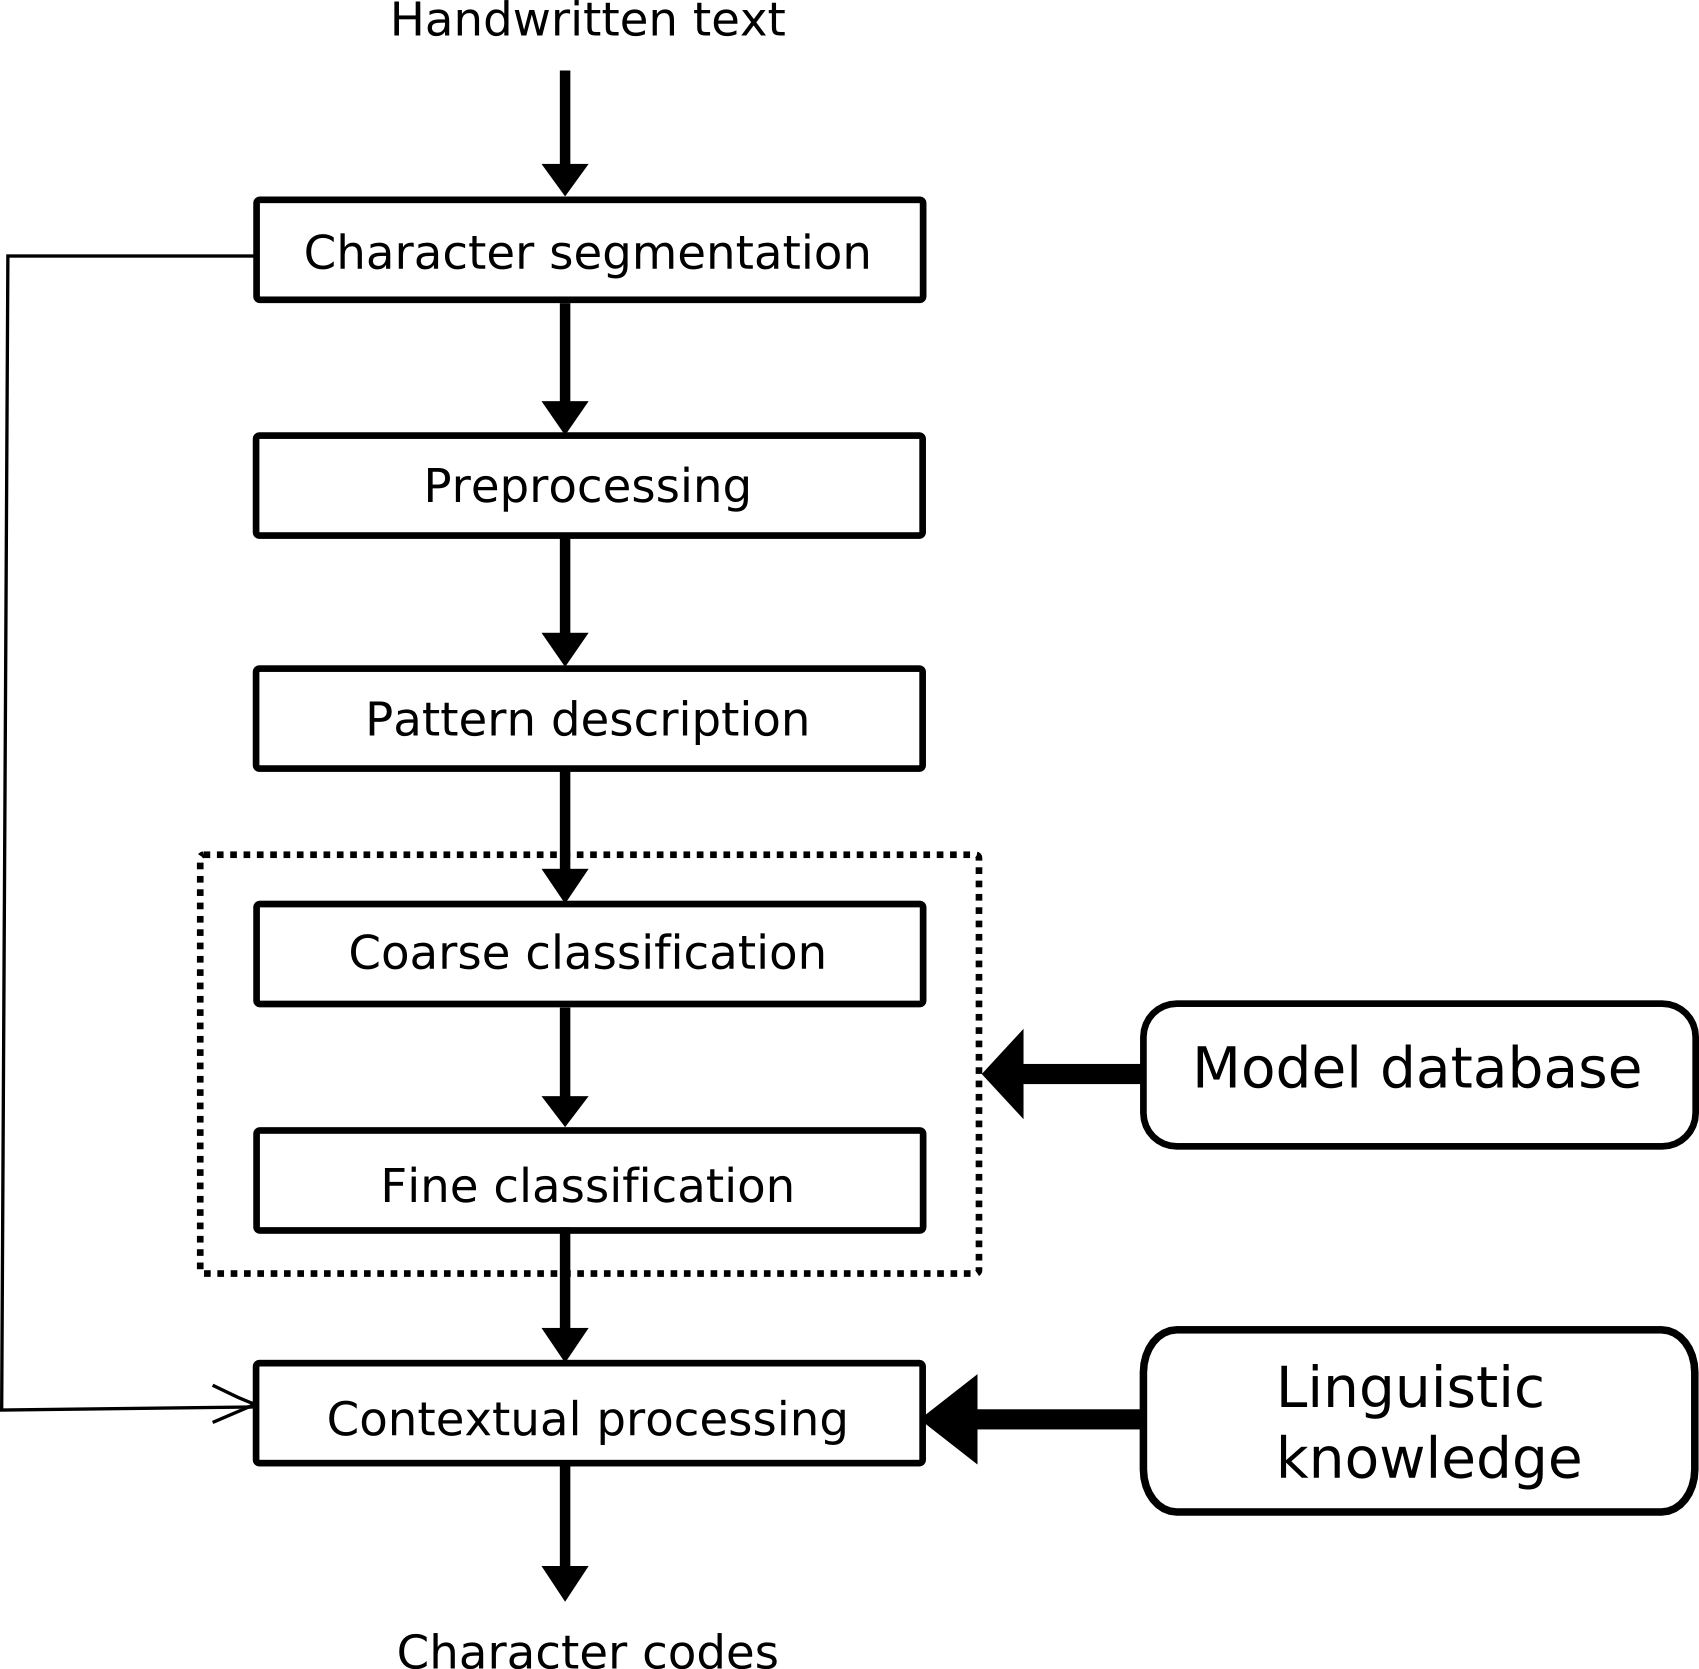
\includegraphics[scale=0.5]{images/olccrSystemOverview.png}
\caption{Overview of an OLCCR system}
\label{fig:olccrsystemoverview}
\end{figure}

A typical OLCCR system is depicted 
after~\shortciteANP{LiuJaegerNakagawa2004}~\citeyear{LiuJaegerNakagawa2004} in 
figure~\ref{fig:olccrsystemoverview}.
The first two steps, character segmentation and preprocessing are virtually
identical to systems dealing with Latin script. The next step, pattern 
representation is not only different from Latin script systems, but it has
great diversity among the different OLCCR systems.
The pattern description is naturally more alike in the systems focusing on 
Latin characters. This is due to the fact that the Latin alphabet is quite 
small, but has more variation concerning writing style, whereas the Chinese 
alphabet has a larger inventory of characters, but less variation in how to 
write a character. The reason for that is that it is widely agreed upon a 
standard stroke sequence for a character, even across country 
borders \shortcite{Nakai2003}.
The next step after the pattern representation is the actual character 
recognition or classification. Different flavours of comparison methods are
applied in different systems, but some systems employ coarse classification 
first, then a fine classification, whereas other systems try to find the 
corresponding character model in a model database in just one step.
The coarse classification is done to reduce the candidate set, the fine 
classification is used to find the best match. There are systems that 
accomplish another step \emph{contextual processing}, which can be regarded 
as an equivalent to postprocessing~\shortcite{LiuJaegerNakagawa2004}.

\subsection{Character Segmentation}
\label{sec:olccr:charactersegmentation}

Character segmentation is a technique that does not apply to OLCCR systems in
the same way it does to HWR systems for other scripts. Each character is
written separately, even in cursive script. In Chinese characters, \emph{cursive}
refers to reduction of lines and lesser pen-up movements within a character.
In e.g. Latin script it usually refers to not lifting up the pen before the end
of a word~\shortcite{Tappert1990}. Therefore character segmentation is often a
trivial task in OLCCR systems, also due to the fact that systems usually only
allow writing in boxes - or, in box-free application, assume horizontal 
character orientation~\shortcite{Nakagawa2008}.

One system attempts to recognise overlaid handwriting characters on a small 
display, allowing continuous writing for the user. That is essentially boxed
writing, but because of the small display, there is only one box in which 
all characters have to be drawn. The system can therefore be regarded as a
continuous character recognition system. In that system, character segmentation 
is not done as a preprocessing step, but during recognition. The system uses 
HMM technique, based on substrokes and segments the characters alongside the 
recognition process~\shortcite{Shimodaira2003}.

The system developed by~\shortciteANP{Nakagawa2008} in~\citeyearNP{Nakagawa2008}
performs continuous character recognition, regardless of the text orientation.
The average character size is estimated from all strokes drawn and the estimate
defines a threshold for the separation of characters.

\subsection{Preprocessing}
\label{sec:olccr:preprocessing}

The preprocessing techniques used in OLCCR systems are mainly the same as the
ones described in section~\ref{sec:preprocessing}, in~\shortcite{Tappert1990}
and in~\shortcite{Santosh2009}. However, since the input devices offer higher 
quality input, less noise reduction is necessary and smoothing is enough to 
remove undesirable points from the input trajectory. Therefore, many OLCCR 
systems limit preprocessing to the other techniques. Data points are reduced
by one of two methods: approximation of lines (by feature points) or 
resampling~\shortcite{LiuJaegerNakagawa2004}.
Size normalisation is realised in most HWR systems, OLCCR systems included.

\subsection{Pattern Description}
\label{sec:olccr:patterndescription}

An important part of each HWR system is the description of the patterns that
need to be recognised. Since the Japanese and Chinese alphabet has a manifold 
character set, pattern representation faces greater difficulty, because confusion
of characters must be avoided.
There are three main types of pattern description in OLCCR systems. The 
classification of characters depends highly on that representation.
In the beginning of research into OLCCR systems, \emph{structural} character 
representation was the natural choice. As systems and computing power evolved, 
\emph{statistical} character representation became more relevant. In order to 
optimise for speed and recognition accuracy, system designers started blending
the two methods to \emph{hybrid statistical-structural} character representation
~\shortcite{LiuJaegerNakagawa2004}. Systems that use statistical character
representation usually store the input patterns in feature vectors. The character
model database holds the parameters for classification.

\subsubsection{Statistical Character Representation} 
\label{sec:olccr:statisticalrepresentation}

In statistical character representation, the central focus lies on transferring
input patterns into feature vectors. The model database contains the same type
of classification information for the characters.
Since each stroke of a character is represented in a feature vector, 
systems are enabled to perform stroke order free recognition. The trajectory
can also be mapped into a 2D image, in order to apply off-line recognition 
features. An on-line version of the direction feature, commonly used in off-line recognition systems, can be found in several systems~\shortcite{Suen2003}. 
Generally, using features and a statistical representation, 
enables the use of several feature extraction techniques that have been 
developed for off-line systems~\shortcite{LiuJaegerNakagawa2004}.

\subsubsection{Structural Character Representation}
\label{sec:olccr:structuralcharacterrepresentation}

Several different approaches have been proposed to structural character 
representation. The most basic version of a structured representation is simple
point sequences. Systems that use point sequences as a representation,
calculate the distance between the strokes. Another approach deals with feature 
point or line segments. Feature points are calculated from the original 
point sequence, which is ideal for characters with mostly straight lines. 
Instead of matching complete point sequences, only feature point sequences need 
to be matched with the character database~\shortcite{LiuJaegerNakagawa2004}.

Using stroke codes for character representation has been adopted by a number of
OLCCR systems. Each of the graphemic strokes of the Kanji stroke inventory is
named. A character representation consists of a stroke sequence of the named
strokes or a relation between the strokes.

\paragraph{Structured Character Representation} 
is a approach where the characters are structured in their graphemic 
subcomponents. \shortcite{Nakagawa2008} employ basic sub patterns and then 
structural information about how these are combined to form a full character.
That way, the dictionary is smaller, because there is only limited number of 
sub patterns and their variations. The sub patterns are not chosen randomly,
but taken from the inherent hierarchical structure of the Hànzì and Kanji.
The characters are organised hierarchically in the way that each one of them
is built from the same set of radicals. Therefore the characters can be 
described as a trees or directed acyclic graphs, using the radical 
representations. In the dictionary, the radicals are shared between the 
characters, reducing the dictionary size 
immensely~\shortcite{LiuJaegerNakagawa2004}. 
There are around 200 radicals but around 3000 Kanji characters in active use in 
the Japanese script. Creating a character representation for each one of them 
is a considerable effort however, using a structured approach can lessen that 
labour-intensive task. \shortcite{Breen2004} proposed a multi-index dictionary 
that bears the potential to support the creation of structured character 
databases. Besides the alleviation of the database creation, the storage space 
used can limited, which will be advantageous when building a system for small 
computing devices.

\subsubsection{Statistical-Structural Character Representation}
\label{sec:olccr:statistical-structuralcharacterrepresentation}

A common example of statistical-structural character representation is the 
\emph{substroke approach}. \shortcite{Nakai2001}, \shortcite{Shimodaira2003}, 
\shortcite{Okumura2005} and others define 8 or more\footnote{Some systems 
distinguish between short and long strokes and thus use 16 stroke types.} stroke 
types, each of which has its own direction and orientation. These are used to
describe input patterns sequentially but also non-sequentially.

In statistical-structural models, characters are described in graph or tree 
structures. The primitives, e.g. the substrokes and their relations to each other
are represented in a probabilistic model. 
Most of the substroke systems use HMMs. The substrokes are represented by nodes
and the transition between strokes is measured probabilistically. Some systems
use points or line segments. Other systems use full strokes or even radicals.
Attempting to avoid stroke-order dependence of the system, often multiple HMMs
are generated with stroke-order variations.
The substroke approach responds to that by hierarchical character models,
such that the stroke order variations can be stored in a 
network~\shortcite{LiuJaegerNakagawa2004}.

\subsection{Classification}
\label{sec:olccr:classification}

%xxx: \shortcite{Plamondon2000}
%xxx: \shortcite{Nakagawa2008}

Classifying an input pattern representation as an entry found in a pattern 
database is the kernel of each pattern recognition application.
Representing data in the same format as the original patterns 
(see~\ref{sec:olccr:patterndescription} is another key task, however the actual
classification is the main piece of software.
In this section, different kinds of classification are reviewed to fit with
the different kinds of pattern description. The two main groups of 
classification methods are reviewed: \emph{structural classification} and 
\emph{probabilistic classification}.
Additionally, a short section about \emph{coarse classification} shows how to
speed up the classification process by preprocessing in the sense of 
classification preprocessing, not to be confused with the data preprocessing
described in section~\ref{sec:preprocessing}.

\subsubsection{Coarse Classification}
\label{sec:olccr:coarseclassification}

Coarse classification is a name for any method that pre-selects characters
to match an input pattern, before the detailed or fine classification is done.
There are different coarse classification methods, but nevertheless the overall
goal of coarse classification remains the same. Increasing the speed of the
classification process.
That appears to be necessary due to large vocabulary size. Comparing an input
pattern with each pattern in the pattern database is a time-consuming process.
Therefore, many system designers subdivide their database into \emph{character
classes}. When a new input pattern needs to be analysed, the system first assigns
a character class and therefore reduces the search space. This coarse 
classification method is called \emph{class set partitioning}. Another method of 
coarse classification is \emph{dynamic candidate 
selection}~\shortcite{LiuJaegerNakagawa2004}.

\paragraph{Class Set Partitioning} methods divide the large set of characters  
into smaller groups - character classes. These groups can be completely disjoint 
or sometimes overlap. The system assigns the input pattern to one or more 
character classes. After that, in the next step of the recognition process, 
the input pattern is compared to the members of the character class it has been 
assigned to. The groups are devised in the database design 
phase~\shortcite{LiuJaegerNakagawa2004}.

\paragraph{Dynamic Candidate Selection} methods calculate a matching score between 
the input pattern and each character class. A subset of character classes is 
selected for further enquiry. ~\shortcite{LiuNakagawa2000} have shown that the 
increase in recognition speed can be achieved without loss of precision by 
choosing a variable number of classes according to a confidence value.
The dynamic grouping can be based on several different factors. For instance
the overall character structure, the basic stroke substructure, the stroke 
sequence~\shortcite{LiuJaegerNakagawa2004}.
Selection the partition classes dynamically is less labour-intensive, because it
avoids the training process or manual division of the character classes.
Stroke number of the input pattern can also be used as a preselection of
characters. Systems that employ structured character representations (see 
section~\ref{sec:olccr:structuralcharacterrepresentation}) can also use radical 
detection. All characters in the database that do not contain the confidently 
detected radical are ruled out from fine classification. However, the radical
detection has a close relation to structural classification (see 
section~\ref{sec:olccr:structuralclassification}) and cannot be done without it.
Another possibility to perform coarse classification is feature vector matching,
where only a subset of the feature vector is compared and thus rules out all
character database entries that do not match~\shortcite{LiuJaegerNakagawa2004}.

\subsubsection{Structural Classification}
\label{sec:olccr:structuralclassification}

Structural classification refers to a set of methods for classification or
character matching that use the internal structure of the character in order to
perform the matching. Input patterns are compared to structural representations
of the candidate character classes.
The one with the minimum distance measure is considered the resulting character.

The different methods of structural classification can be grouped as follows:\\
\emph{Stroke matching} or \emph{stroke correspondence}, 
\emph{elastic matching} or \emph{DP matching (dynamic programming)}, 
\emph{relational matching} and \emph{knowledge-based matching}.
Stroke matching compares the strokes that have been drawn with the strokes of the
character model in the character database. Elastic matching is performed on 
ordered stroke sequences and contains stroke deformation techniques. 
Relational matching considers the strokes and the interstroke relationships, 
whereas stroke matching only considers the strokes, but not their relations 
to each other. \emph{Hierarchical matching} and \emph{deformation methods} are 
connected to these approaches in an orthogonal fashion, i.e. they can be combined
with the approaches mentioned above.

\paragraph{Hierarchical Matching} can improve recognition speed, because parts 
of the recognition and representation are done only once for several characters.
That approach would of course not be possible without the hierarchical 
composition of the Kanji characters. The accuracy of that approach is limited in
the way that the accuracy of the recognition depends on the accuracy of the
radical recognition. However, when a radical has been recognised correctly, 
the classification can succeed by traversing a decision tree or 
network~\shortcite{LiuJaegerNakagawa2004}.

\paragraph{Deformation Methods} deform the input pattern in a way to better match
with a character representation from the database. In order to do that a 
deformation vector field is computed, based on the stroke correspondence.
Then the prototype is deformed by local affine transformations in order to fit 
the input pattern.

\paragraph{Stroke Matching} is a technique where a distance between the input 
strokes and the strokes in the database are calculated. The distance between an
input pattern and a character in the database is the sum of the between stroke
distances. When the input strokes are reordered according to domain-specific 
rules, alternative stroke orders can be matched. The domain-specific rules 
contain linguistic information such as the stroke order precedence.
Alternatively, there can be several database entries for the same character with
varying stroke orders. Defining these rules is a labour-intensive 
task~\shortcite{LiuJaegerNakagawa2004}.

\paragraph{Elastic Matching} does not differ much from the general elastic matching 
techniques described in section~\ref{sec:curvematching}. Elastic matching 
searches for the ordered correspondence between primitive symbols, such as 
coordinate points or line segments. During that process the algorithm seeks to
minimise the edit distance (\emph{Levenshtein distance}). A popular elastic 
matching technique is called \emph{Dynamic time warping} (DTW), which is used by
many different systems, especially the concerned with HWR for scripts that
have rather curvy characters like Tamil \shortcite{Niels2005}, \shortcite{Joshi2004b} or Devanāgarī \shortcite{Joshi2005}, but has also been applied to HWR of
latin-based alphabets \shortcite{Negussie2008}, \shortcite{Vuori2001}.
\shortcite{Niels2004} and \shortcite{Joshi2004a} have done research into which 
elastic matching approach is suitable for HWR, as well as, if DTW is useful for 
that task at all. Both conclude that the method bears advantages, because 
certain problems concerning handwritten input, such as stroke length, or number 
of sample points can be dealt with.

\paragraph{Relational Matching} systems search for correspondences between element sets. That is, for example the spatial relationships between strokes in a set of 
strokes in a character representation. Since the stroke order within radicals
tends to be invariant, it is possible to perform elastic matching for the strokes
within the radical and use relational matching for the strokes on a character 
level. Just like elastic matching and stroke matching, relational matching can
be performed by systems focusing on character patterns or radicals.
The advantage of relational matching over elastic matching is that it is 
stroke-order independent. Since the relationship constraint improves the accuracy
of the matching, relational matching also has an advantage over stroke matching.
However, it is computationally complex and therefore slower than the other 
two methods~\shortcite{LiuJaegerNakagawa2004}.

\paragraph{Knowledge-Based Matching} utilises the knowledge of the internal 
structure of characters. The knowledge is formulated and represented as heuristic
rules or constraints. The constraints reduce the search space of structural 
matching efficiently. Radical detection and stroke reordering have been performed
by rule-based methods. The rules hold the information of permitted basic strokes
for a character or fixed spatial feature of strokes.
Building knowledge-based systems can be laborious, because of the tasks of 
acquiring and organising the knowledge. However, even simple heuristics have
proved to be valuable. Some heuristics can be acquired in an automatic fashion,
or from corpus studies, for example statistical distribution of stroke order for
characters. With rule-based heuristics, the overall recognition accuracy of
systems based on other classification methods can be 
improved~\shortcite{LiuJaegerNakagawa2004}.

\subsubsection{Probabilistic Classification}
\label{sec:olccr:probabilisticclassification}

The use of probabilistic methods for classification has increased. Many modern 
OLCCR systems use probabilistic methods successfully. For example, the stroke-type
probability can help computing the between-stroke distance. Alternatively,
if the prototype strokes are modelled as Gaussian density functions, the 
matching score of an input pattern respective to a character model can be 
computed using the joint probability of constituent 
strokes~\shortcite{LiuJaegerNakagawa2004}.

\paragraph{HMM-based Classification} has been a popular method in recent years of
research in OLCCR systems. The recognition task is the decoding of the 
observed sequence (i.e. the input sequence) into the most probable state 
sequence. This is done with the Viterbi algorithm, that is very popular for
these types of decoding tasks, such as automated 
translation~\shortcite{KoehnHoang2007}. Radicals can be represented in HMMs and 
therefore be shared between different characters in the character database.

\shortcite{Hu1996} have incorporated HMMs into a stochastic language model for 
Latin characters. \shortcite{Tokuno2002} employed a substroke model for cursive
Kanji and Hiragana handwriting recognition. Their model contains 
contend-dependent substrokes and their character model therefore needs 25 HMMs
as opposed to one for each character. The substroke approach became popular,
and has been used by \shortcite{Nakai2001}. In a follow-up article, 
\shortcite{Nakai2003} propose the automated generation of a dictionary for 
stroke-order free OLCCR. That approach is as well based on substroke HMMs.
\shortcite{Shimodaira2003} propose a handwriting recognition interface for 
wearable computing. In their approach the HWR has do be done overlaid, i.e. the
user draws sequential characters in the same box. The resulting segmentation
problem is solved by using substroke HMMs, where recognition is done in parallel
with segmentation. In order to achieve that, a stochastic bi-gram language model
is combined with the HMMs.
Another system~\shortcite{Okumura2005} uses not only the pen-direction feature 
of the other substroke-based HMM approaches, but additionally incorporates the 
pen-coordinates into the system. This is done at the inter-state transitions of 
the HMM, whereas the pen-direction feature is utilised at the intra-state 
transitions.

\subsection{Postprocessing}
\label{sec:olccr:postprocessing}

\subsubsection{Contextual Processing During Recognition}
\label{sec:olccr:contextualprocessingduring}

OLCCR systems, focus on finding the appropriate candidate for an input pattern.
Once the correct character has been found the task is solved. Most systems
deal with extraction of features and classification or matching, resulting in 
scores for individual characters. There are systems that have to deal with 
multiple character input. That can make the problem more complex, 
for example when dealing with overlaid handwriting and the accompanying 
segmentation problem~\shortcite{Shimodaira2003}. 

In Japanese, it is possible to write from left to write in lines, 
while the lines go from to to bottom. It is also possible, to write from top 
to bottom in columns, while the columns go from right to left. 
The task of recognising multiple character input becomes more difficult,
when attempting to recognise Japanese handwriting without assumptions about the
writing direction~\shortcite{Nakagawa2008}. 
However, it is possible to make use of the linguistic context for contextual 
processing of already recognised character classes.
The context can provide additional information about which character class is
the most suitable among a selection of possibilities with their scores.
Also, geometric features like size, location or aspect ratio can support the 
segmentation process. 

For page-based recognition processes - especially in the case of off-line 
recognition, but also when handwriting input can be placed freely on some
input device with a stylus-based or touch display - it is important to integrate
the segmentation and the recognition modules. Frequently, segmentation can not
be done unambiguously before the recognition~\shortcite{LiuJaegerNakagawa2004}.

Some segmentation ambiguities need to be solved during the recognition process.
Usually, the systems generate some candidate character classes and verify them
by their geometric features, the recognition results and also linguistic 
knowledge. The candidates can be represented in a network, where the edges denote
combinations or segments that build up the candidate pattern.
Each path in the pattern represents a segmentation of the input and its 
recognition result. A dynamic programming search yields the path with the highest
probability value. Linguistic knowledge can be used to verify the path or
can be inserted into the path scores~\shortcite{LiuJaegerNakagawa2004}.

\subsubsection{Contextual Processing After Recognition}
\label{sec:olccr:contextualprocessingafter}

Linguistic processing of system results after segmentation and recognition
is called \emph{postprocessing}. For instance, based on the recognition result,
other candidate characters can be given, due to statistical information about 
confusion of characters. That procedure reduces the risk of excluding the
true class from the candidate set.

Additionally to that, there are systems that ruthlessly exploit linguistic 
knowledge in dictionaries or character-based or word-based n-grams 
models. Word-based n-gram models usually provide syntactic or semantic classes, 
for example parts of speech. Using n-gram models involves dividing text into 
words and some degree of morphological analysis. It is beneficial to use 
writer-specific dictionaries. Generally, linguistic postprocessing improves
the accuracy of the recognition~\shortcite{LiuJaegerNakagawa2004}.

